\documentclass[a4paper,11pt]{article}
\usepackage{cv}

\usepackage[utf8]{inputenc}
\usepackage{listings}
\usepackage{color}
\usepackage{amsthm}
\usepackage[english]{babel}
 
\newtheorem{theorem}{Theorem}

\definecolor{codegreen}{rgb}{0,0.6,0}
\definecolor{codegray}{rgb}{0.5,0.5,0.5}
\definecolor{codepurple}{rgb}{0.58,0,0.82}
\definecolor{backcolour}{rgb}{0.95,0.95,0.92}
\lstdefinestyle{mystyle}{
    backgroundcolor=\color{backcolour},   
    commentstyle=\color{codegreen},
    keywordstyle=\color{magenta},
    numberstyle=\tiny\color{codegray},
    stringstyle=\color{codepurple},
    basicstyle=\footnotesize,
    breakatwhitespace=false,         
    breaklines=true,                 
    captionpos=b,                    
    keepspaces=true,                 
    numbers=left,                    
    numbersep=5pt,                  
    showspaces=false,                
    showstringspaces=false,
    showtabs=false,                  
    tabsize=2
}
\lstset{style=mystyle}

\name{\hspace{0.3cm}Jipeng, Sam}
\info{CSE-6010 Assignment 3: \\[0.2cm]
      Graph Analytics Part1}
      
\bibliography{rjhpubs}
\begin{document}
\maketitle
\thispagestyle{empty}


\section{Literature Search And Expected Results--Jipeng}
\begin{theorem}
\emph{(Size of Largest Components In A Random Graph)}
\label{Lagrange}
Consider a random graph $G \in G_{n,p}$ where $p=c/n$ for some constant c. Then:
\begin{enumerate}
\item If $c<1$, then a.a.s., the largest component of G has size $O(log(n))$, or more exactly, at least $\frac{3ln(n)}{(1-c)^2}$. 
\item If $c>1$, then a.a.s., G has a largest component of size $O(n)$. It is a unique "giant" component of size $(1+o(1))\beta n$, where $\beta$ is the unique solution in $[0,1]$ to the equation $\beta+e^{-\beta c}=1$. All other components have size $O(log(n))$.
\item If $c=1$, then a.a.s., G has a component of size $O(n^{\frac{2}{3}})$.
\end{enumerate}
The phrase "a.a.s"(asymptotically almost surely) is used to denote an event that holds with probability tending to 1 as $n \to \infty$.
\end{theorem}

According to this theorem, the expected size of the largest component can be plotted. There is no exact expected size value. We can evaluate the correctness by judging whether the size is consistent with $log(n)$, $n$ or $n^{\frac{2}{3}}$ in probability. 

\begin{figure}[H]
  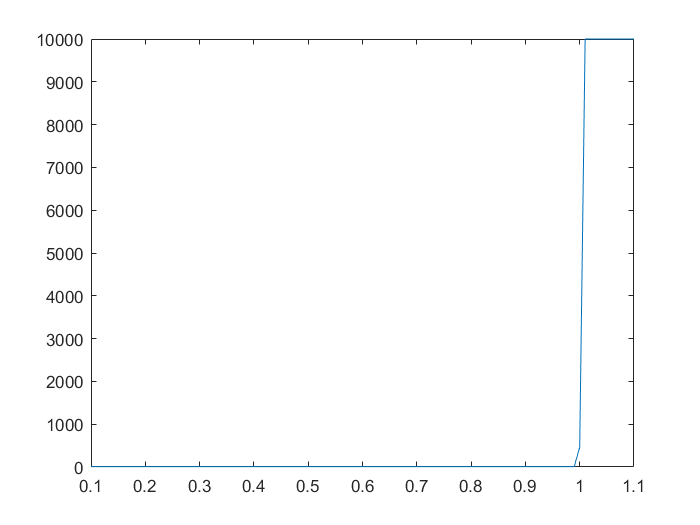
\includegraphics[width=3.8in]{plot1.png}
  \caption{Expected Largest Component Size in Probability}
\end{figure}


\section{Graph Analysis--Sam}


\begin{thebibliography}{9}
\bibitem{latexcompanion}
  S. Janson, T. Luczak, and A. Rucinski.
  \textit{Random Graphs}.
  Wiley, 2000.
\end{thebibliography}  
\end{document}
